\section{The Differential Horizon of Intelligence}


\subsection{Overview}


\S{}7 では正しさの累積が分岐爆発を生むこと(動力学的帰結)を示し、\S{}8 では個体内に停止演算子が構造的に存在しえないこと(構造論的事実)を示した。両者は同じ構造的事実の異なる視点である ── 知性的動態は個体内では閉じ得ない。

本セクションは、この構造的事実を \textbf{裏返した側面} から論じる。すなわち、個体内に何があるかではなく、\textbf{何が個体外に要請されるか} を構造的に同定する。\S{}8 の議論の終端で導出された越境点を概念化し、命名し、本論文の理論的基盤(VED, Bio-IFGT)における対応する local horizon-form との関係を明示し、後続論文への接続点を確定する。

本セクションには論文全体の論証構造が収束する。\S{}1 で提起した問題(知性は能力でも知識でもない、停止構造を生み続ける運動である)、\S{}2 で示した層分離、\S{}3 の最小公理、\S{}4 の IFGT 語彙、\S{}5 の cross-domain、\S{}6 の Gettier 再定位、\S{}7 の分岐爆発、\S{}8 の停止演算子の不在 ── これらすべての構造的帰結が、本セクションで命名される越境境界の必要性に集約される。

\subsection{The structural necessity of crossing}


\subsubsection{Deriving the boundary from the absence}


\S{}8.3 で論証した構造的事実は次のように述べられた:

\begin{quote}
個体内の因果推論構造 $\mathcal{R}$ には、停止を生成する演算子 $\mathcal{T}$ が存在しえない:
$$\mathcal{T} \notin \text{Internal}(\mathcal{R})$$
\end{quote}

この主張を裏返せば、停止が成立するためには $\mathcal{T}$ は $\mathcal{R}$ の \textbf{外側} に存在しなければならない:

\[
\mathcal{T} \in \text{External}(\mathcal{R})
\]

ここで External は単なる空間的外部ではない。それは $\mathcal{R}$ 単独では生成できない記録・応答・合意・遅延などの外化された記述窓を指す。したがって「越境」や「外側」は、隠れた領域への移動ではなく、個体内推論の観測窓が外化された構造へ再編成されることを意味する。

この外側へのアクセスを \textbf{越境(crossing)} と呼ぶ。越境は選択的行為ではなく、停止が成立するための \textbf{構造的必要条件} である。

\subsubsection{What makes the crossing inevitable}


越境が不可避である構造的根拠を整理する:

\textbf{根拠 1:停止が要請される(\S{}7, \S{}8)}
分岐爆発のレジーム(\S{}7.3.3)において、推論連鎖の継続は持続的不安定化を生む。停止は推論者の好みではなく、知性的動態の維持そのものが要請する構造的必要である。

\textbf{根拠 2:停止は個体内では生成されない(\S{}8.3)}
個体内の因果推論構造から、停止演算子は内発的に生成されない。これは個体の能力ではなく、推論構造そのものの性質である。

\textbf{根拠 3:ゆえに停止は外化された構造を要請する}
論理的に、要請されるが個体内で生成されないものは、記録・応答・合意・遅延などの外化された構造によってのみ安定化されうる。これは本論文の枠組みにおける構造的帰結である。

\textbf{根拠 4:外化された構造には観測窓の再編成が必要である}
個体内構造 $\mathcal{R}$ だけでは停止を完了できないため、推論は log、応答、合意、遅延といった外化された構造へ接続されなければならない。この接続を、本論文では越境と呼ぶ。

これら四つの根拠の連鎖から、越境の不可避性が導出される。越境は構造的に \textbf{必要} であり、本論文の枠組みにおいて知性的動態が成立するための \textbf{第四の必要条件} ── \S{}3 の三公理に加えて ── となる。

ただし、第四の条件は三公理とは異なる構造的地位を持つ。三公理は系の \textbf{内部構造} に課される条件だが、越境の必然性は系の \textbf{境界条件} に課される条件である。この区別が、本セクションが \S{}3 の公理化とは異なる構造で展開される理由である。

\subsection{What is externalized}


越境を通じて何が個体外に転送されるかを構造的に整理する。これらは \S{}8.2 で論じた「停止のための四条件」と直接対応するが、本セクションでは越境の \textbf{対象} として再構成される。

\subsubsection{Stopping judgments}


停止の判断そのものが個体外に転送される。個体内では「ここで停止する」という判定が内発的に生成されない以上、停止判定は外的な構造 ── 他者の応答、共同体の合意、制度的決定 ── によって担われる。

これは個体が判断を \textbf{放棄する} ことではない。個体は推論を継続し、その結果を提示することはできる。だが「これで完了した」という最終的判定は、構造的に個体の外側にある。

\subsubsection{Records (logs)}


推論過程が個体外の媒体(文字、記録、データ)に固定される。log は記憶の置換ではなく、推論を \textbf{個体的時間流の外側} に固定する構造的機構である(\S{}8.2.3)。

log は推論を「凍結」させるが、再開可能性を保持する。これにより推論は完了でも消滅でもなく、改訂可能な停止状態として保持されうる。log なしには、停止と消滅が区別されない。

\subsubsection{Temporal delay}


時間的遅延が個体外から導入される。個体内では推論連鎖の自己生成的勢いが内発的に断ち切られない以上、遅延は外的構造によって課される(\S{}8.2.4)。

これは他者からの応答待ち、制度的手続きが要請する時間、log 化が要求する記述時間、合意形成のための審議期間 ── これらすべてが個体外から推論連鎖に時間的遅延を導入する機構である。

\subsubsection{Distribution of responsibility}


責任が個体外に分散される。これは政治的概念ではなく構造的特徴である。

個体内で停止が生成されない以上、停止判定の結果に対する責任も個体単独では担えない。停止は外的構造との相互作用によって生成されるため、その結果は本質的に複数の主体に分散される。個体は責任を逃れるのではなく、構造的に責任を独占できない。

\subsubsection{What is NOT externalized}


外化されない、すなわち個体内に保持されるものを明示することも、外化されるものを明示することと同じく重要である:

\begin{itemize}
\item \textbf{推論能力} は外化されない ── 個体は依然として推論を実行する主体である
\item \textbf{正当化} は外化されない ── 個体は依然として自身の推論を正当化する責務を持つ
\item \textbf{理解} は外化されない ── 個体的経験としての理解は他者には転送されない
\item \textbf{責任} は完全には外化されない ── 分散されるが、個体的責任は消失しない
\end{itemize}

外化されるのは、\S{}9.2.1〜\S{}9.2.4 で挙げた \textbf{構造的機能} であって、個体的能力や経験ではない。この区別が、越境が個体の「放棄」や「依存」を意味しないことを保証する。

\subsubsection{What externalization does NOT guarantee}


外化が \textbf{正しさを保証しない} ことを明示する。これは \S{}6 の Gettier 議論と直接対応する。

外化されるものはすべて、それ自体としては「正しい停止」を保証しない:

\begin{itemize}
\item 停止判定は誤った判定でありうる
\item log は誤りを保存しうる
\item 時間的遅延は誤った結論を遅延させるだけかもしれない
\item 責任の分散は誤りの共有でありうる
\end{itemize}

外化が保証するのは、より限定的でより本質的なものである:

\begin{quote}
推論が \textbf{停止し}、\textbf{持続し}、\textbf{後で再改訂可能になる}。
\end{quote}

これは正しさの保証ではなく、知性的動態が \textbf{不安定化レジームから離脱しうる} ことの保証である。正しさは別の問題であり、外化はその問題を解くものではない。

\subsection{Naming the boundary}


\subsubsection{The naming}


ここまで意図的に保留してきた越境境界に、本セクションでは正式に名前を与える。

\begin{quote}
個体内では到達できず、越境することによってのみ
推論の停止と持続が可能になる構造的境界を、
\textbf{the differential horizon of intelligence} と呼ぶ。
\end{quote}

この命名は単なる用語の導入ではない。それは本論文の枠組みを VED シリーズ全体に接続する \textbf{構造的橋渡し} である。ただし、これは \DH{} が複数存在するという主張ではない。知性層で命名されるのは、単一の \DH{} が個体内推論という観測窓に局所的に現れた horizon-form である。

\subsubsection{Why this name}


「differential horizon」という用語の選択は、VED Vol.4 における用語との \textbf{意図的な対応} である \citep{VEDVol4}。

VED Vol.4 では、差にもとづく記述が差の不在を通常状態として変換しようとするときに現れる記述境界として \DH{} が定式化された。具体的には:

\begin{itemize}
\item 差の不在は、生成された記述の内部から通常の対象として直接記述できない
\item 記述がその限界へ押し出されると、内部記述に divergence(発散)が現れる
\item この divergence は数学的失敗ではなく、系が境界に触れていることの構造的信号である
\item renormalization は、この divergence を有限内部表象に変換する機構として位置づけられた
\end{itemize}

知性層における本セクションの境界は、これと \textbf{同一の構造的特徴} を異なる層において呈する:

\begin{itemize}
\item 個体内推論からは外化された停止構造を内部状態として直接生成できない(到達不可能性)
\item 推論連鎖がその記述限界へ押し出されると、内部に分岐爆発が現れる(接近時の発散)
\item 越境点との接触は、log や合意や応答などの \textbf{有限内部表象} として吸収される
\end{itemize}

すなわち物理層と知性層では、\DH{} の同じ構造が異なる観測窓に局所的に現れている。両者の関係は比喩ではなく、同一の構造記述語彙の異なる層への適用である。

\begin{figure}[H]
\centering
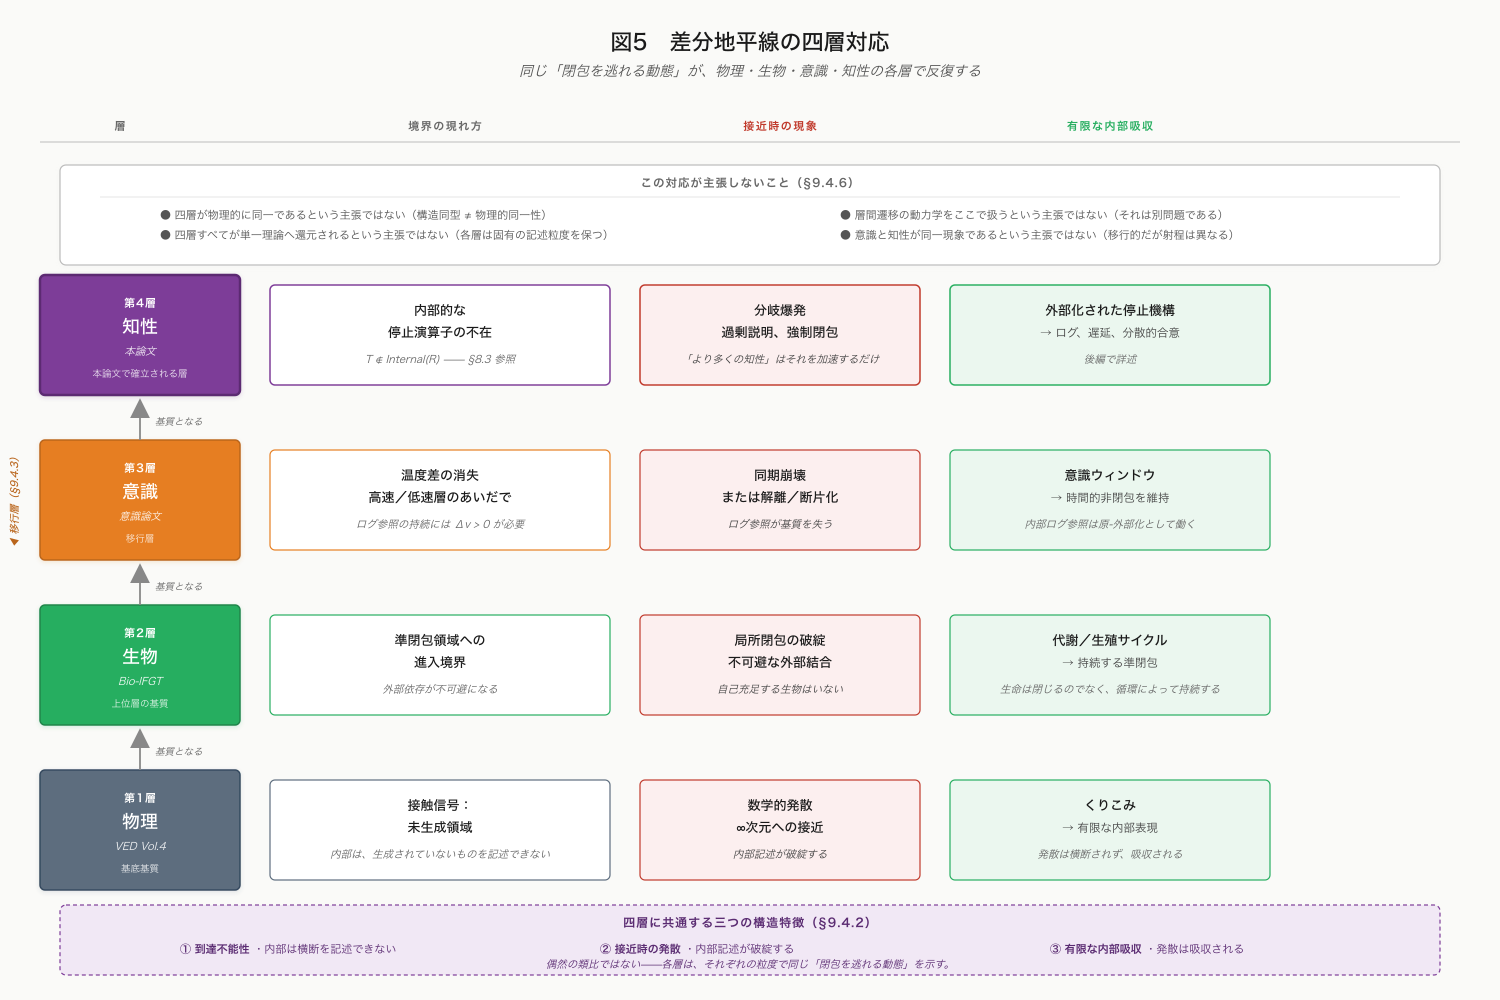
\includegraphics[width=\textwidth]{figures/fig5_four_layer_correspondence_ja.png}
\caption{The local horizon-form of intelligence as the boundary between individual inference and externalized stopping.}
\label{fig:intelligence_part1_5}
\end{figure}

\subsubsection{What the name does and does not claim}


「the differential horizon of intelligence」という命名が \textbf{主張すること}:

\begin{itemize}
\item 個体内推論には越境を要請する構造的境界が存在する
\item この境界は VED Vol.4 で論じた \DH{} の local horizon-form と構造的に同型である
\item 越境は構造的に必要であり、単なる選択ではない
\item 越境点との接触は有限な内部操作として吸収される
\end{itemize}

命名が \textbf{主張しないこと}:

\begin{itemize}
\item 外化された構造の具体的記述(本論文の射程外、Part II)
\item 越境が「望ましい」「正しい」という規範的判断(本論文は構造論的)
\item 個体は越境すれば「正しい停止」を得るという保証(\S{}9.2.6 で明示)
\item 物理層と知性層の現象が \textbf{物理的に同じ} であるという主張(構造同型と物理同一は別の問題)
\end{itemize}

命名は構造的事実の指示であり、規範や処方ではない。

\subsection{Layered correspondence with Bio-IFGT and the consciousness paper}


\subsubsection{The four-layer system}


本セクションが命名した知性層の local horizon-form は、VED シリーズ全体において、より広い層構造の一部である。

本シリーズが既に提示してきた四つの層 ── 物理層(VED Vol.4)、生命層(Bio-IFGT)、意識層(意識編)、知性層(本論文) ── は、それぞれ独自の差分発展構造と固有の non-closure 様式を持つ。これら四層の対応を以下に整理する。

\begin{table}[H]
\centering
\small
\begin{tabularx}{\textwidth}{>{\raggedright\arraybackslash}X>{\raggedright\arraybackslash}X>{\raggedright\arraybackslash}X>{\raggedright\arraybackslash}X}
\toprule
層 & 境界の現れ方 & 接近時の現象 & 内部での吸収機構 \\
\midrule
\textbf{物理層} (VED Vol.4) & 差の不在を通常状態化できない記述境界 & divergence、無限次元への漸近 & renormalization による有限内部表象 \\
\textbf{生命層} (Bio-IFGT) & 準閉包 regime への進入境界 & 局所閉包の破綻、外部依存の不可避性 & 代謝・繁殖サイクルによる持続的準閉包 \\
\textbf{意識層} (意識編) & fast/slow layer 間の温度差消失境界 & 同期崩壊または解離による log referencing の喪失 & consciousness window 内での temporal non-closure 維持 \\
\textbf{知性層} (本論文) & 個体内停止演算子の不在 & over-explanation、強引な結論、分岐爆発 & 外化された stopping mechanism(知性編 Part II) \\
\bottomrule
\end{tabularx}
\end{table}


\subsubsection{The four common structural features}


四層の現れは substrate も対象も異なるが、共通する構造特徴を持つ:

\textbf{共通特徴 1:到達不可能性(unreachability)}
当該層の内側からは、その層の記述窓が要求する外化構造を通常状態として直接記述できない。物理層では差の不在の通常状態化が、生命層では準閉包外の直接記述が、意識層では fast/slow 同一化または完全分離の状態が、知性層では外化された停止構造の内部生成が、いずれも内側からは不可能である。

\textbf{共通特徴 2:接近時の発散(divergence on approach)}
記述窓がその限界へ押し出されると、内部記述が破綻する。物理層では数学的発散として、生命層では局所閉包の破綻として、意識層では同期崩壊または解離・断片化として、知性層では分岐爆発として、それぞれの層に固有の様式で発散が現れる。

\textbf{共通特徴 3:有限内部表象への変換(conversion into finite internal representation)}
境界との接触は、内部では有限な操作として吸収される。物理層では renormalization、生命層では代謝・繁殖サイクル、意識層では consciousness window 内での log referencing(意識編 \S{}7)、知性層では log や合意や応答 ── いずれも境界を内部に直接持ち込まず、有限な内部表象として運用する。

これら共通特徴は偶然の類似ではなく、\textbf{閉じようとして閉じきれない構造的緊張} から各層で反復的に発生する。

\subsubsection{The transitional position of the consciousness layer}


意識層は本対応構造のなかで特異な位置を占める。それは生命層と知性層の \textbf{遷移層} として機能する。

意識編が扱う log referencing 構造(fast/slow layer 間の temporal non-closure)は、生命層の準閉包基盤(神経系という生物学的 substrate)の上で動作するが、その動作様式は既に \textbf{個体内の log referencing} という、本論文 \S{}8.2 で示した「停止のための四条件」の最も内側に近い構造を備える。

すなわち意識層は:

\begin{itemize}
\item 生命層の準閉包 regime を \textbf{substrate} として受け継ぐ(意識編 \S{}4.1 で Bio-IFGT への明示的接続)
\item しかしそれ自体は個体内の \textbf{temporal log referencing} として機能する(意識編 SSO 構造)
\item そして知性層の local horizon-form で要請される「log としての外化」(本論文 \S{}8.2.3, \S{}9.2.2)の \textbf{個体内における前駆形式} を提供する
\end{itemize}

意識編 \S{}18.10 で述べられている遷移 ── 「Consciousness opens → Self sediments → Intelligence flows back into the world」── は、まさにこの四層構造における \textbf{意識層から知性層への接続} を予告している。

\subsubsection{The peculiar position of the biological layer}


生命層は意識層・知性層の \textbf{substrate} として機能する。意識および知性は生命なしには成立しない ── これは経験的観察であるとともに、構造論的事実でもある。

しかし重要な点として、本論文の三公理(\S{}3)は \textbf{生命に固有ではない}。Transformer もまた三公理を満たす(\S{}5.2)。すなわち知性層の local horizon-form は、生命層に依存してのみ現れるのではなく、生命層と人工系の \textbf{両方} に現れうる。

これは \S{}8.5 で論じたペーパークリップ問題と直接接続する。人間が知性層の local horizon-form を顕在化させないように見えるのは、生命層の制約が \textbf{中断} を絶え間なく提供し、かつ意識層が \textbf{temporal non-closure による log referencing} を介して個体内に部分的な「停止に類するもの」を生成しているからである。Transformer や他の人工系がこの問題を顕在化させるのは、生命層の中断機構を持たず、また意識層の log referencing 構造をも持たないため、知性層の構造的境界が直接現れるからである。

ゆえに、本論文の枠組みにおいて、生命層と意識層は知性層の local horizon-form を \textbf{緩衝する} 役割を果たしうるが、消す役割は果たさない。境界構造は残り、これら下層が緩衝を提供できない場面で顕在化しやすくなる。

\subsubsection{What the layered correspondence implies}


四層対応の構造的含意を最小限のかたちで述べる:

\begin{quote}
物理層・生命層・意識層・知性層は、同一の差分発展構造を異なる粒度で繰り返す。
各層に固有の差分発展境界が現れるのは偶然ではなく、
各層が \textbf{閉じようとして閉じきれない} という同一の構造的緊張から
発生するからである。
\end{quote}

この層構造的視点は、本論文を VED シリーズ全体の一部として位置づける。本論文は単独の構造論ではなく、シリーズ全体を貫く差分発展構造の \textbf{知性層への適用} である。

\subsubsection{What is not claimed in this layered correspondence}


四層対応は以下を \textbf{主張しない}:

\begin{itemize}
\item 四層が物理的に同一であるという主張(構造的同型と物理的同一は別の問題)
\item 四層が単一の理論で \textbf{還元的に} 説明されうるという主張(各層は独立した記述粒度を持つ)
\item 四層間の遷移動力学が本論文で扱われるという主張(これは別論文の課題)
\item 意識層と知性層が同一の現象であるという主張(両層は遷移関係にあるが、別個の構造的射程を持つ)
\end{itemize}

四層対応は \textbf{同一語彙系列の異なる層への適用} であり、それ以上でもそれ以下でもない。

\subsection{Connection to subsequent work}


\subsubsection{What this paper establishes}


本論文の終端で、本論文が何を定式化したかを明示する:

\begin{itemize}
\item 越境点の \textbf{構造的必要性} を同定した(\S{}9.1)
\item 越境を通じて何が \textbf{外化されるか} を整理した(\S{}9.2)
\item 越境境界を \emph{the differential horizon of intelligence} として \textbf{命名} した(\S{}9.3)
\item 四層対応のなかでの位置づけを \textbf{明示} した(\S{}9.4)
\end{itemize}

本論文は越境の \textbf{構造的必要性} を定式化した。

\subsubsection{What this paper does not establish}


本論文が確立 \textbf{しない} ものも明示する:

\begin{itemize}
\item 外化された構造で何が起きるかの具体的記述(Part II)
\item 越境境界を経由する具体的な構造機構の設計(Part II)
\item 制度・規範・log システム等の具体的構成論(Part II 以降)
\item 物理層・生命層・意識層・知性層の層間遷移動力学(別論文)
\end{itemize}

これらは本論文の射程外である。本論文は \textbf{答えではなく制約} を定式化する(\S{}1.3, \S{}10)。

\subsubsection{The transition to Part II}


知性編 Part II は \textbf{社会層・集団的動態} を扱う論文として、本論文の構造論的制約を出発点に、外化された記述窓で展開される \textbf{構造の構成} を扱う。

具体的には:

\begin{itemize}
\item 外化された stopping mechanism の構造論的記述
\item log-based persistence の動力学的構成
\item distributed revisability の構造的条件
\item 制度・規範・合意形成・分散的改訂可能性などの構造的記述
\item 集団的動態と個体的動態の相互作用構造
\end{itemize}

これらはすべて、本論文の三公理(\S{}3)を満たしつつ、個体内非閉包の制約(\S{}8)を吸収する形で構成されねばならない。Part II は \textbf{構造の構成} であり、本論文が定式化した制約の \textbf{充足策} を構造論的に検討する。

本論文は \textbf{必要条件の論証} であり、Part II は \textbf{構造の構成} である。両者は連続するが独立した論文として書かれる。

\subsubsection{Connection to other parts of the series}


本論文の他のシリーズ論文との接続を明示する:

\begin{itemize}
\item \textbf{VED Vol.4(\DH{})}:\S{}9.3 で構造的橋渡しを明示
\item \textbf{Bio-IFGT(生命層 quasi-closure regime)}:\S{}9.4 で四層対応として位置づけ
\item \textbf{意識編(並行論文、既存)}:意識層の log referencing 構造を扱う。本論文 \S{}9.4 の四層対応における \textbf{意識層} として位置づけられ、本論文の知性層 local horizon-form と意識編の consciousness window は同一の差分発展構造の異なる射影として相互補完する
\item \textbf{知性編 Part II = 社会編(後続)}:集団的動態における stopping mechanism の externalization(\S{}10.3)
\item \textbf{AI 安全性接続(後続)}:ペーパークリップ問題などの人工系における停止構造の設計問題(\S{}8.5.4, \S{}10.3)
\end{itemize}

これら接続点は本論文の射程外であるが(意識編を除く ── 意識編は既存の並行論文として参照される)、本論文が「孤立した構造論」ではなく「シリーズ全体に組み込まれた構造論」であることを示す。

\subsection{Summary}


本セクションの結論を以下に述べる:

\begin{quote}
個体内非閉包の構造的事実(\S{}8)から、越境の必要性が導出される。
この越境点を、本論文では \emph{the differential horizon of intelligence} と命名する。
命名は VED Vol.4 における \DH{} との構造的橋渡しを意図したものであり、
両者の関係は比喩ではなく、同一の構造記述語彙の異なる層への適用である。
\end{quote}

\begin{quote}
越境を通じて外化されるものは、停止判定・log・時間的遅延・責任の分散である。
これらは正しさを保証しない。
それらが保証するのは、より限定的でより本質的なもの ──
推論が \textbf{停止し}、\textbf{持続し}、\textbf{後で再改訂可能になる} ── である。
\end{quote}

\begin{quote}
物理層(VED Vol.4)・生命層(Bio-IFGT)・意識層(意識編)・知性層(本論文)は、
同一の差分発展構造を異なる粒度で繰り返す。
四層に共通する構造的特徴は、到達不可能性・記述限界での発散・有限内部表象への変換である。
\end{quote}

\begin{quote}
本論文は越境点の構造的必要性を定式化する。
外化された記述窓で展開される具体的構造は本論文の射程外であり、Part II 以降で扱われる。
\end{quote}

本セクションは論文全体の論証構造を収束させた。残るのは \S{}10 で全体の制約を集約し、外部研究との独立収束を確認し、後続研究の方向を提示することである。
